\section{Shaders}

\subsection{Cube Map}

  \begin{figure}[H]
    \centering
    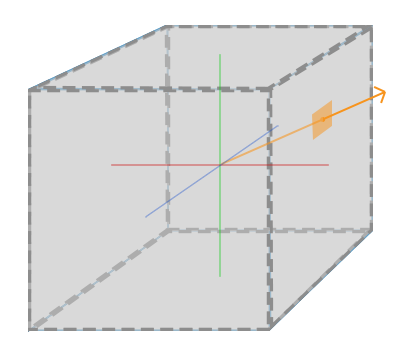
\includegraphics[width=0.4\columnwidth]{images/textures/shaders/cube-map.png}
  \end{figure}

  A cube texture is made of 6 textures, each representing a face of a cube.
  Then, a vector 3 $ \vec{R} $ is used to obtain the color of a point on the
  cube texture

  \begin{itemize}
    \item The largest magnitude of $ \vec{R} $ determines the side to use
    \item Other two components determine the 2D coordinate on the chosen side
    at which to pick the color
  \end{itemize}
